\chapter{Software that has the Quality Without A Name - Federico Mena Quintero}
\todo{bio}
When I was learning how to program, I noticed that I frequently hit the same
problem over and over again: I would often write a program that worked
reasonably well, and even had a good structure, but after some time of modifying
it and enhancing it, I could no longer tweak it any further. Either its
complexity would overwhelm me, or it would be so tightly written that it allowed
no room for expansion, like a house where you cannot build up because it has a
sloping roof, and you cannot build to the sides because it has a wall all around
it.

As I got better, I learned to deal with complexity. We all learn how to do that
with various tools and techniques: abstraction, encapsulation,
object-orientation, functional techniques, etc. We learn how various techniques
let us write broader programs.

However, the problem of having a program that was too tight or too intertwined
to modify still persisted.  Sometimes I had what I thought was a beautiful
design, but modifying it in any way would ``make it uglier'' and I did not want
that. Other times I had something with so many interconnected parts, that I just
could not plug anything else into it or the whole thing would fall down under
its own weight.

Some years ago the whole \textit{Refactoring} craze started, but I did not pay
much attention to it. I said, sure, it is a way to clean up your code, but so
what?  I already know how to take a chunk of code and turn it into a function; I
already know how to take similar chunks of code and turn them into derived
classes. I already know how to write mostly-clean code. What's the big deal?

I dismissed \textit{Refactoring} as something suited to less-experienced
programmers; as some nice recipes for cleaning up your code, but nothing that
you could not discover yourself.

The same thing happened to me with \textit{Design Patterns}. I thought they were
just giving pompous names like Singleton and Strategy to the everyday kinds of
structures one would naturally put in a program. Maybe my ego as a programmer
was too inflated to consider those works seriously. But then, something
happened.

\section*{Christopher Alexander's work}

Some years ago, my wife and I bought a small, one-storey house and we wanted to
expand it. We were thinking of having a child, so we needed more space. I needed
a real home-office, not just a leftover alcove where my desk and bookcases
barely fit. As avid cooks, we both needed a kitchen that was larger and more
comfortable than the one the house had. My wife needed a Room Of Her Own.

We did not want to pay for an expensive architect, and neither of us knew
anything about construction.  How would we design our house?

At times, while browsing the web, I'll sometimes remember that I have seen the
name of a certain author before, or the title of a book, or something like that.
I may have not really paid attention to it in the past, but somehow, the more
times I see the same thing mentioned, the more likely it is that I will get
interested enough in it to actually see what it is about. ``Oh, several people
have already mentioned this name or this book; maybe I should check it out.''

That is just what happened with the name of Christopher Alexander. I had read
that he was a peculiar architect (of real-world buildings, not software),
somehow connected to the software world through object-oriented techniques. As I
started reading about his work, I became tremendously interested in it.

In the 1970s, Christopher Alexander was a mathematician/architect teaching at
the University of California, Berkeley. He and a group of like-minded architects
went to various places around the world, trying to see if there were reasons for
why there are human-built places in the world (cities, towns, parks, buildings,
houses) where it is very pleasant to be, those that are comfortable, livable,
and \textit{nice}, and some places where this is not the case. The pleasant
places were present in all of the traditional architectures of the world -
European, African, Asian, American - which pointed to the idea of being able to
extract common factors from all of them.

Alexander and his team distilled their findings into a list of good
architectural patterns, and published three books: \textit{The Timeless Way of
Building}, where they describe the philosophy and method of good architecture;
\textit{A Pattern Language}, which I will describe next; and \textit{The Oregon
Experiment}, where they detail the design and construction of a university
campus with their method.

\section*{A Pattern Language}

A pattern is a recurring problem when designing and building things, with a
discussion of the forces that shape the problem, and with a solution that is in
turn connected, almost recursively, to other super- or sub-patterns.  For
example, let us consider the INTIMACY GRADIENT, an important pattern in the book
(patterns are spelled in capital letters throughout the book for easy
identification, so I will do the same):

\subsection*{INTIMACY GRADIENT}

\paragraph*{Super-patterns and preamble:}
... if you know roughly where you intend to place the building wings - WINGS OF
LIGHT, and how many stories they will have - NUMBER OF STORIES, and where the
MAIN ENTRANCE is, it is time to work out the rough disposition of the major
areas on every floor.  In every building the relationship between the public
areas and private areas is most important.

\paragraph*{Statement of problem:}
Unless the spaces in a building are arranged in a sequence which corresponds to
their degrees of privateness, the visits made by strangers, friends, guests,
clients, family, will always be a little awkward.

\paragraph*{Discussion:}
I will not quote all of it. But for example, consider an apartment where you can
only reach the bathroom by first crossing the bedroom. Visits are always awkward
because you feel like you need to tidy up your room first, if you intend your
visitors to be able to use the WC! Or consider an office, where you do not want
a quiet work space to be right next to the reception, because then it will not
be quiet at all - you want it to be more private, towards the back.

\paragraph*{Summary of the solution:}
Lay out the spaces of a building so that they create a sequence which begins
with the entrance and the most public parts of the building, then leads into the
slightly more private areas, and finally to the most private domains.

\paragraph*{Sub-patterns to consult:} COMMON AREAS AT THE HEART. ENTRANCE ROOM
for houses; A ROOM OF ONE'S OWN for individuals.  RECEPTION WELCOMES YOU for
offices, HALF-PRIVATE OFFICE at the back.

The patterns get quite specific, but they never impose a style or an actual
shape for the result. For example, there is a pattern called OPEN SHELVES. Deep
cupboards make you put things behind other things, so you can not see them nor
reach them. They also have a big footprint. Cupboards that are one-item-deep
automatically stay tidy, and you always know at a glance where everything is.
Things that you use frequently should not be behind doors.

So you can see the essence of design patterns: good, tested recipes that do not
constrain your implementation in unnecessary ways.  The patterns do not mandate
a particular style, nor include superfluous decorations: the book does not tell
you, ``make this shape of flourishes in the handrails''; instead it tells you,
``a house should have its rooms placed such that sunlight enters them according
to the time of the day in which they are most used - East for the bedrooms in
the morning, West for the living room in the afternoon''.

I had gotten a copy of \textit{A Pattern Language} shortly before starting the
expansion of our house. The book was a revelation:  \textbf{this} was the way to
approach the design of our house, and now we could do it ourselves instead of
paying a lot of money for an inadequate solution. We were able to make up a
rough plan for our house, and then figure out smaller details as the
construction went on. This is the kind of book that, as you read it, manages to
confirm intuitive ideas that you half-knew you had - the kind of book where you
find yourself saying, ``of course, this is completely how I thought it should
be'' all the time.

\textit{Design Patterns}, the well-known book by Gamma et al, took direct
inspiration from Alexander's architectural patterns. They wanted to do the same
thing: to make a list of problems that appear frequently when programming, and
to present good solutions for them, that would not constrain your implementation
unnecessarily.

One thing that I realized while reading \textit{A Pattern Language} - a valuable
thing from both lists of patterns, the architectural and the software one, is
that they give us a vocabulary to talk about how things are constructed. It is
much more convenient to say, ``this object has listeners for its properties'',
than ``this object lets you hook callback functions that are called when its
properties change''. What I thought were only pompous names, are in fact ways to
express knowledge in a compact form.

\section*{The Quality Without A Name}

Much of Alexander's discussion of patterns and their philosophy refers something
which he calls the ``Quality Without A Name''. You know places with the Quality
Without A Name. It is present in the coffee shop where you like to go to read,
because the afternoon light hits it at just the right intensity, and there are
comfortable seats and tables, and somehow it always is packed with people and
yet you do not feel overcrowded. It is present in the corner in a park where a
tree shades a bench, maybe there is some water running, and no matter if it
rains or if it is sunny, it always seems to be a pleasure to be there. Think of
a Hobbit House, where everything is at hand, everything is comfortable, and
everything is lovingly made.

A thing or place has the Quality Without A Name if it is comfortable, has
evolved over time in its own terms, is free of inner contradictions, does not
try to draw attention to itself, and seems to have archetypal qualities - like
if it were the way that thing was supposed to be built. Most importantly,
Alexander asserted that this is an objective quality, not a subjective one, and
that it can be measured and compared. Although this seems like a very vague
definition, that is as far as Alexander was able to take it during this first
phase of his work. The real revelation would come later.

As programmers, we have all seen beautiful programs at some point. Maybe they
are the examples in \textit{Programming Pearls}, a beautiful book which every
hacker should read. Maybe you have seen a beautifully implemented algorithm that
exudes rightness.  Maybe you remember a very compact, very legible, very
functional, very correct piece of code. That software has the Quality Without A
Name.

It became clear to me that I had to learn to write software that attained the
Quality Without A Name, and Alexander's frame of mind was the right starting
point for this.

\section*{The ticket booth}

Alexander's PhD dissertation, which was the basis for his book \textit{Notes on
the Synthesis of Form} from 1964, tried to mathematize design by defining it as
a progression from a series of requirements to a final result, through an
analysis of the forces that shaped the design.

Let me quote Richard Gabriel, of whom I will talk more later, when he describes
the time when Alexander was trying to design a ticket booth based on his
mathematical ideas:
\begin{quote}
Alexander says [about the Quality Without A Name]:
\begin{quote}
It is a subtle kind of freedom from inner contradictions. (Alexander 1979)      
                                                                   \end{quote}
This statement reflects the origins of his inquiry into the quality. It started
in 1964 when he was doing a study for the [San Francisco] Bay Area Rapid Transit
(BART) system based on the work reported in Notes on the Synthesis of Form
(Alexander 1964), which in turn was based on his Ph.D. dissertation. One of the
key ideas in this book was that in a good design there must be an underlying
correspondence between the structure of the problem and the structure of the
solution - good design proceeds by writing down the requirements, analyzing
their interactions on the basis of potential misfits, producing a hierarchical
decomposition of the parts, and piecing together a structure whose
\begin{quote}
structural hierarchy is the exact counterpart of the functional hierarchy
established during the analysis of the program. (Alexander 1964)\end{quote} 
Alexander was studying the system of forces surrounding a ticket booth, and he
and his group had written down 390 requirements for what ought to be happening
near it. Some of them pertained to such things as being there to get tickets,
being able to get change, being able to move past people waiting in line to get
tickets, and not having to wait too long for tickets. What he noticed, though,
was that certain parts of the system were not subject to these requirements and
that the system itself could become bogged down because these other forces -
forces not subject to control by requirements - acted to come to their own
balance within the system. For example, if one person stopped and another also
stopped to talk with the first, congestion could build up that would defeat the
mechanisms designed to keep traffic flow smooth. Of course there was a
requirement that there not be congestion, but there was nothing the designers
could do to prevent this by means of a designed mechanism.                      
                                                                                
                                                                                
                                                                                
                                                                                
                                                                                
                                                                                
                                                                                
                                                                                
                                                                                
                                                                                
                                                                                
                                                                              
\end{quote} 
As a programmer, does this sound familiar?  You can make a beautiful, thorough
design, that crumbles down when you actually build it because things emerge that
you did not anticipate. This is not a failure of your design, but of something
else! Richard Gabriel goes on:
\begin{quote}
Alexander said this:
\begin{quote}
So it became clear that the free functioning of the system did not purely depend
on meeting a set of requirements. It had to do, rather, with the system coming
to terms with itself and being in balance with the forces that were generated
internal to the system, not in accordance with some arbitrary set of
requirements we stated. I was very puzzled by this because the general
prevailing idea at the time [in 1964] was that essentially everything was based
on goals. My whole analysis of requirements was certainly quite congruent with
the operations research point of view that goals had to be stated and so on. 
What bothered me was that the correct analysis of the ticket booth could not be
based purely on one’s goals, that there were realities emerging from the center
of the system itself and that whether you succeeded or not had to do with
whether you created a configuration that was stable with respect to these
realities.\end{quote}                                                           
                                                                                
  \end{quote}
And that is the core of the problem:  how do you create a configuration that is
stable with the realities that emerge from itself as you build it?

\section*{The Nature of Order}

Although Christopher Alexander knew that he had produced something valuable with
his investigation and catalog of patterns, he was not completely satisfied.
Where had the patterns come from? Could we make new patterns from scratch, or
must we be content with what traditional architecture has managed to evolve so
far? Are patterns necessary at all?  How can we better define, and evaluate or
measure, the Quality Without A Name?

Alexander spent the next twenty years researching those questions. By studying
the actual process by which good built environments had been created, he
discovered that processes of a certain kind are essential to creating good
towns, or buildings, or any man-made thing in fact. He arrived at the following
conclusions:
\begin{itemize}
 \item Nature creates things that all have about 15 properties in common (I will
show you later). This happens solely through natural processes - standard
physics and chemistry - although it is not quite clear why very different
processes produce similar results.
 \item Traditional architectures, or towns which just evolved over time, also
have those properties. You can derive all the patterns in \textit{A Pattern
Language} by following a certain process based on those properties.
 \item Each property can also describe a transformation to the existing space.
 \item The only way to achieve good design is by using those transformations,
one at a time.
\end{itemize}
This was published in 2003-2004 in four volumes titled \textit{The Nature of
Order}.

\section*{The fifteen properties}

The first book in \textit{The Nature of Order} deals with fifteen properties
that appear in all natural systems. I will summarize them very briefly; see the
references for pictures and more extensive explanations.
\begin{itemize}
 \item \textbf{Levels of scale:} There is a balanced range of sizes. You do not
have abrupt changes in the sizes of adjacent things. Elements have fractal
scale.
 \item \textbf{Strong centers:} You can clearly identify parts of the space or
structure.
 \item \textbf{Thick boundaries:} Lines delimit things. In living systems, edges
are the most productive environments (e.g., all the critters that live at the
edge of the water).
 \item \textbf{Alternating repetition:} High/low, thick/thin, shape A and shape
B. Things oscillate and alternate to create a good balance.
 \item \textbf{Positive space:} Space is beautifully shaped, convex, enclosed.
It is not leftover space. Think of how a Voronoi diagram has cells that grow
outward from a bunch of points, or how a piece of corn has kernels that grow
from tiny points until they touch the adjacent kernels.
 \item \textbf{Good shape:} The sails of a ship, the shell of a snail, the beak
of a bird. They attain the optimal shape for their purpose, which is beautiful.
 \item \textbf{Local symmetries:} The world is not symmetrical at large. But
small things tend to be symmetrical, because it is easier that way. Your house
is not symmetrical, but each window is.
 \item \textbf{Deep interlock and ambiguity:} The crooked streets of old towns.
Axons in neurons. It is hard to separate figure and ground, or foreground and
background.  Two strong centers are made stronger if a third center is placed
between them, so that it belongs to both.
 \item \textbf{Contrast:} You can distinguish where one thing ends and the next
one begins, because they do not fade into each other.
 \item \textbf{Gradients:} Things fade into each other where they need to.
Concentrations in solutions, snow or earth banks, the wires that support a
bridge. The way bandwidth decreases as you move away from the backbone.
 \item \textbf{Roughness:} The world is not frictionless and smooth.
Irregularities are good because they let each piece adapt perfectly to its
surroundings, rather than being an exact copy that may not fit as well.
 \item \textbf{Echoes:} Things repeat and echo each other. Things are unique in
their exact shape, but the general shapes repeat over and over.
 \item \textbf{The void:} Sometimes you get a big blank area for quietness of
form. A lake, a courtyard, a picture window.
 \item \textbf{Simplicity and inner calm:} Things are as simple as possible, but
no simpler.
 \item \textbf{Non-separateness:} Everything depends on everything else. You can
not separate a fish from the pond and the aquatic plants. You can not separate a
column from the base of the building.
\end{itemize}

\section*{Structure-preserving transformations}

The second book in \textit{The Nature of Order} describes how each of those
properties also defines a transformation. For example:
\begin{itemize}
 \item \textbf{Thick boundaries:} You can sometimes transform something
beneficially by adding a boundary to it. You plant a hedge around a garden,
which then serves as beauty, as a wind-break so that strong winds do not damage
the garden, and as a productive system on its own. In a graphical user
interface, scrollable boxes without a frame are hard to distinguish from the
window's background (think of all white web pages with text entry boxes that do
not have a frame). You put a cornice at the top of a building, so that you do
not get an abrupt transition between the building and the sky.
 \item \textbf{Local symmetries:} Small parts of built things are easier to
build symmetrically; because they are turned on a lathe, because they need
access from both sides, because they fold like a book. Making things
asymmetrical just to be interesting takes extra work and it is harder to make
them work well.
 \item \textbf{Positive space:} Feeling too exposed when in your desk?  Add a
waist-high bookshelf beside you to delimit your space, but not to completely
close you off. Does your user interface feel like a lot of leftover space after
you place the controls?  Make the controls surround the usable space instead.
\end{itemize}
Each of these is a structure-preserving transformation. You make a change in the
existing structure not by tearing it down and remaking it, but by tweaking one
thing at a time according to those properties as transformations.

In software terms, it turns out that this is what much of \textit{Refactoring}
is about, when you translate the concepts to code. Refactoring is just applying
structure-preserving transformations, or as Martin Fowler (the author of
\textit{Refactoring}) would put it, behavior-preserving transformations. You do
not change what the program does; you just change how it is built internally,
piece by piece.

By extracting a chunk of code and putting it in a function with a name, you are
essentially adding a thick boundary around that code, and creating a strong
center. By removing a global variable and adding class variables, you are
allowing for roughness, as every instance can now have a different value in that
variable, as needed. By having a producer/consumer, or notifier/listener, you
have local symmetries, deep interlock and ambiguity, and good shape.

Richard Gabriel, one of the principal figures in Common Lisp, studied how to
apply Alexander's theories to software (and also to poetry, and isn't code
similar to poetry after all?).  He gives the following example:
\begin{enumerate}
 \item Imagine that you write a PhoneCall class. This is a latent center, not as
strong as it could be.
   \begin{figure}[h!]
     \centering
     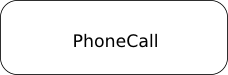
\includegraphics[scale=0.6,keepaspectratio=true]{./usability/federico1.png}
   \end{figure}
 \item Gerard Meszaros, in \textit{Pattern: Half Object + Protocol} suggested
that you should split that into half calls tied by a protocol.
   \begin{figure}[h!]
     \centering
     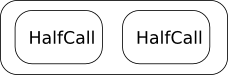
\includegraphics[scale=0.6,keepaspectratio=true]{./usability/federico2.png}
   \end{figure}
 We attain a local symmetry, we make a strong center, and get levels of scale.
 \item Now make a diagram of that:
   \begin{figure}[h!]
     \centering
     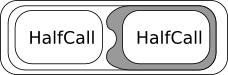
\includegraphics[scale=0.6,keepaspectratio=true]{./usability/federico3.png}
   \end{figure}
 You have local symmetry, levels of scale, boundaries, deep interlock and
ambiguity - and this is where Meszaros left things.
 \item Richard Gabriel then suggests strengthening the centers that exist by
applying other structure-preserving transformations. What about the latent
center in the middle?
   \begin{figure}[h!]
     \centering
     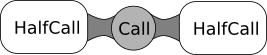
\includegraphics[scale=0.6,keepaspectratio=true]{./usability/federico4.png}
   \end{figure}
 You add an explicit boundary (Call) that ties the HalfCalls. This improves the
local symmetries, retains deep interlock and ambiguity, and it is composable.
 \item Yes, composable.
   \begin{figure}[h!]
     \centering
     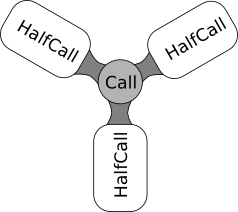
\includegraphics[scale=0.6,keepaspectratio=true]{./usability/federico5.png}
   \end{figure}
 Multi-way calls, conference calls, happen all out of applying
structure-preserving transformations.
\end{enumerate}
Probably every programmer keeps a mental picture of the program he is creating
or modifying - the hard part of modifying code that you did not write is forming
that mental picture in the first place. When you work to make the code present a
more beautiful picture, your code becomes better - and Alexander gives us a good
way to do that.

\section*{The fundamental process}

Over a long argument, Alexander explains why following this process of applying
structure-preserving transformations is the \textbf{only} way to achieve a good,
functional design. This is not just for buildings, but for everything we
construct. It does not matter if you start with an existing program or building
or city, or whether you are starting from scratch. We mimic nature's own
evolutions and regenerative processes, but we do it faster.
\begin{enumerate}
 \item Start with what you have - an empty lot, or an already-built building, or
a program that looks ugly and is hard to use.
 \item Identify the centers that exist in that space. Find the weakest center or
the least coherent.
 \item See how to apply one or more of the fifteen structure-preserving
transformations to strengthen that weak center. Does it need to be delimited?
Does it need to be blended with its surroundings? Does it need more detail? Does
it need to be de-cluttered?
 \item Find the new centers that are born when you apply the transformation to
the old center. Does the new combination make things stronger? Prettier? More
functional?
 \item Ensure that you did the simplest possible thing.
 \item Go back to the beginning for the next step.
\end{enumerate}
A super-simple summary would be: find the bad parts, make them better in the
simplest way possible, test the results, iterate.

Alexander is not keen on destroying things just to rebuild them in a different
way.  You should  not demolish parts of a town to rebuild it; you should improve
it gradually. In software, it is well-known that you should not rewrite things
just because you do not understand them anymore. Tearing things down makes you
lose all the knowledge you had embodied in the thing you are destroying, even if
it looks ugly in its current state.

Similarly, Alexander is against making detailed, up-front designs. He gives a
good argument of why pre-made designs can not work well in the end: because you
can not predict absolutely everything that will come up during construction or
implementation; because you will miss details of the environment into which your
creation will live; because Nature itself is not pre-ordained, and rather it
grows organically and mercilessly evolves things until they manage to survive by
themselves.

In this fashion, you do not design the whole user interface, or the whole
structure, for a big program in a single step. You go from big to small or small
to big (levels of scale); you test each part individually until it is good
(strong centers); you make sure the parts are not too disconnected from each
other (non-separateness). You move a few widgets where they are easier to reach,
or where they are closer to the data to which they refer. You remove some frames
and separators to reduce clutter. Above all, you continually evaluate what you
created against real users and real use cases, so that you empirically test
things against reality, not against castles in the sky.

\section*{A Name for the Quality}

Over the course of \textit{The Nature of Order}, Alexander manages to show that
environments or structures that are built according to that method all end up
having the Quality Without A Name. He calls this \textbf{living structure}. It
can be measured and compared. It no longer has no name; we can now speak of
environments with more or less living structure than others, or of programs with
more or less living structure than others - and we strive to make have more of
that property.

I just called this essay, "Software that has the Quality Without A Name" because
it sounds more mysterious that way.

I can not claim to know the perfect way of designing and writing software now,
but at least I have a good method grounded on what produces good things
elsewhere. It worked for my house, and so far I have seen it work very well for
my software. I hope it works well for you, too!


\section*{References}
\begin{itemize}
 \item Christopher Alexander, \textit{A Pattern Language}. Online version at
\url{http://vasarhelyi.eu/books/A\_pattern\_language\_book/apl.htm}
 \item Christopher Alexander, \textit{The Nature of Order}. Terrible web page at
\url{http://www.natureoforder.com}
 \item Photos and drawings of the fifteen properties of life -
\url{http://www.livingneighborhoods.org/ht-0/fifteen.htm}
 \item Richard Gabriel, \textit{Patterns of Software}. A beautiful, wide-ranging
book on software development, Christopher Alexander's ideas, and the search for
good techniques for writing software. Online version at
\url{http://dreamsongs.com/Files/PatternsOfSoftware.pdf}
 \item Richard Gabriel, \textit{Christopher Alexander: the search for beauty}. A
very good presentation of Christopher Alexander's ideas and an exposition of
patterns in the software world.
\url{http://dreamsongs.com/Files/AlexanderPresentation.pdf}
 \item Richard Gabriel, \textit{The Nature of Order: the post-patterns world}.
Another very good presentation, subsequent to the previous one, that explains
the Fifteen Properties of Life, the Fundamental Process, and how this relates to
software. \url{http://dreamsongs.com/Files/NatureOfOrder.pdf}
\end{itemize}
